\documentclass{article}
% NeurIPS style (same family as Blier & Ollivier 2018, arXiv:1802.07044): single column, Times, numbered references.
\PassOptionsToPackage{numbers,sort&compress}{natbib}
\usepackage[preprint]{neurips_2024}
\usepackage[utf8]{inputenc}
\usepackage[T1]{fontenc}
\usepackage[hidelinks]{hyperref}
\usepackage{url}
\usepackage{booktabs}
\usepackage{amsmath,amssymb}
\usepackage{graphicx}
\usepackage{subcaption}
\usepackage{xcolor}
\usepackage{microtype}
\newcommand{\Dh}{\hat D}
\newcommand{\cell}[1]{\texttt{#1}}
\graphicspath{{../figures/}}

\title{Programs for a Frozen Machine:\\ The Description Length of Language and Task in Optimized Prefixes}
\author{%
  Georgii Sirotenko\\
  Heidelberg University\\
  \texttt{georgii.sirotenko@stud.uni-heidelberg.de}
}

\begin{document}
\maketitle

\begin{abstract}
A frozen language model is a fixed machine; a soft prefix that makes it perform a task is a program for that machine, and the shortest such program is a model-relative description length of the task. We measure that length for a frozen Qwen2.5-1.5B base model over a grid of three tasks (translation from English, factual recall, sentence continuation) and three output languages (Russian, German, English), in two units: prefix slots and variational bits under a bits-back code. Four findings. (i)~Slots are not a description length: translation saturates at one slot, one trained slot beats the natural-language prompt everywhere, and a conditioning string is worth less than a slot. (ii)~In bits, a translation program costs about 500~bits at 10\% excess loss, a Russian recall program five times that, and English recall most of all; continuation has nothing to compress. (iii)~In bits, neither task nor language is the cheap modifier of the other, and sharing does not compress: under a common protocol one centre per task with language deviations and one centre per language with task deviations cost the same within 25\% at matched hyper-parameters, a language given a task costs what a task given a language costs (about 200 bits for translation, 3,200 for recall), and the task-centred hierarchy costs 1.5 times eight independent programs (parity on translation, 1.9 times on recall); the preregistered 37\% advantage of the task-centred nesting was a selection artefact. The asymmetry is in the mechanism: recall programs are language-specific, do not compose zero-shot and are read deep in the network, whereas translation programs are read almost entirely in the first block; inside a hierarchical prefix the language deviation is read again at blocks 16--17, which the task centre is not. (iv)~The variational objective selects compact programs but the standard optimiser does not find them: a conservative step size and checkpoint selection on the full objective lower the measured frontier by 20--71\% with fewer runs, which turns the open problem of \citet{shaw2026bridging} into a recipe at this scale. All numbers regenerate from the released tables.
\end{abstract}

\section{Introduction}
Prompt tuning \citep{lester2021power} and prefix tuning \citep{li2021prefix} adapt a frozen language model by optimising a few continuous vectors prepended to the input. Read as engineering, these vectors are parameters. Read through the lens of algorithmic information theory they are programs: the frozen model is the interpreter, the prefix is the program, the input is the data and the target is the result. \citet{shaw2026bridging} make this reading precise, showing that prompt tokens form a program tape for a Transformer interpreter and that the variational code length of a prompt is an asymptotically optimal description-length objective. \citet{cosma2026prompting} define prompting complexity as a model-relative, resource-bounded Kolmogorov complexity. Both papers measure programs; neither asks how the program for a multilingual task is organised.

This paper asks that question. For a frozen model $M$, task $t$ and output language $l$, let $K_M(t,l)$ be the length of the shortest prefix that performs $t$ in $l$ at a chosen distortion. How is $K_M(t,l)$ split between telling the model which task to perform and which language to produce? Are the two parts separable, so that a task part and a language part can be assembled? How far apart are the programs for different cells, and do they cluster by task or by language? Where in depth does the model read each part? And is the measurement itself trustworthy: does gradient descent find the short programs that the objective prefers?

Our contributions are a measurement design and five results. The design (Section~\ref{sec:framework}) fixes two units, slots and bits, one normalised distortion, two preregistered operating points, and a hierarchical variational prefix whose centre and deviations put task bits and language bits in the same currency. The results (Sections~\ref{sec:results}--\ref{sec:opt}) are the four findings of the abstract plus a negative one: the information-distance matrix over cells has no cluster structure at one seed. Every number is recomputed from released tables by a notebook that runs in under a minute.

\section{Related work}
\paragraph{Description length of models and probes}
\citet{hinton1993keeping} introduced the variational (bits-back) code for network weights; \citet{blier2018description} compared variational and prequential codes for deep networks and found the prequential one far shorter; \citet{voita2020information} used prequential coding to measure what a probe learns. We use both codes: variational for the rate of a prefix and prequential for the distance between prefixes.

\paragraph{Soft prompts as programs}
\citet{shaw2026bridging} give the universality construction and the adaptive prior we build on, and report that the objective selects compressible solutions that random-initialisation training fails to find. \citet{cosma2026prompting} measure shortest prompts, discrete and soft, as a complexity. \citet{mu2023gist} compress instructions into gist tokens; \citet{vu2022spot} treat learned prompts as task embeddings that predict transfer; \citet{vykopal2025soft} combine soft language prompts with task adapters. \citet{khashabi2022prompt} show that a working soft prompt need not read as words, which is why every claim here is functional: transfer, composition, conditioning or intervention, never a nearest-token reading.

\paragraph{Task and language inside the model}
Task vectors \citep{hendel2023context} and function vectors \citep{todd2024function} show that a task can be carried by one hidden vector. \citet{wendler2024llamas} and \citet{dumas2025separating} locate a language-agnostic concept representation in the middle blocks with language resolved later; our patching probes test where a learned task part and a learned language part are read.

\section{Measurement framework}\label{sec:framework}
\paragraph{Interpreter, program, distortion}
The prefix $P\in\mathbb R^{k\times d}$ occupies the first $k$ positions of the input embedding sequence; the model's weights, tokenizer and format are fixed. Distortion is the teacher-forced code length $L$ of the target in bits per target token. To compare across cells we normalise per cell,
\begin{equation}
\Dh=\frac{L-L_{\text{floor}}}{L_{\text{none}}-L_{\text{floor}}},
\end{equation}
where $L_{\text{none}}$ is the no-prefix loss and $L_{\text{floor}}$ the better of a per-cell LoRA fine-tune and the best prefix run. The operating points $\Dh\le0.25$ and $\Dh\le0.10$ were preregistered from a development pilot; $\Dh\le0.05$ is reported as exploratory. All claims are relative to one model: orderings, differences and ratios within it.

\paragraph{Two units}
\emph{Slots} are the number $k$ of prefix positions; the slot complexity $k^\ast$ is the smallest $k$ reaching an operating point, found by sweeping $k$ with free, unpenalised vectors. \emph{Bits} are the description length of the prefix under a prior: each slot is a diagonal Gaussian posterior $q=\mathcal N(\mu,\mathrm{diag}\,\sigma^2)$, trained with its own noise, and its rate is $\mathrm{KL}(q\,\|\,\pi_0)/\ln 2$ with $\pi_0$ a diagonal Gaussian fitted to the model's token-embedding matrix (bits-back). The rate--distortion frontier of a cell is the smallest rate among runs that reach an operating point, over $k$ and the KL weight $\beta$. Distortion of a variational prefix is scored on posterior samples, because the sample is the coded object (Section~\ref{sec:opt} shows what goes wrong when the posterior mean is scored instead).

\paragraph{Hierarchy}
To put task bits and language bits in one currency, a group of cells (the languages of one task, or the tasks of one language) is coded as a centre $c\sim q_c$ with rate $\mathrm{KL}(q_c\,\|\,\pi_0)$ plus one deviation $\delta_m\sim q_m$ per member with rate $\mathrm{KL}(q_m\,\|\,\mathcal N(0,\tau^2\sigma_0^2 I))$, $\tau=1$ in units of the prior scale, so that a deviation costs the same per unit of displacement as a whole prefix. The member's prefix is $c+\delta_m$; the loss is the mean member NLL plus $\beta$ times the centre rate amortised over all members' tokens and the deviation rate over the member's own.

\paragraph{Derived measurements}
\emph{Composition}: one tied task part per task and one tied language part per language, concatenated, trained on all cells or with cells held out and assembled zero-shot. \emph{Distance}: $K_M(a\mid b)$ as the prequential cost of training from cell $b$'s prefix toward cell $a$ over a fixed budget, symmetrised and divided by the from-scratch costs \citep{bennett1998information,li2004similarity}. \emph{Mechanism}: the hidden states at the prefix positions of a trained prefix patched into the attention input of one block of a run with a random prefix, for every block; the recovered loss relative to the full effect is the fraction of the program read at that block. \emph{Regime 2}: per-example vectors replacing the input, with and without the task prefix.

\section{Experimental setup}
\paragraph{Model, data, grid}
Qwen2.5-1.5B base \citep{qwen2.5}, frozen, bfloat16 on an A100. Translation and continuation use FLORES+ (dev split for training and selection, devtest for reporting); recall uses mLAMA \citep{kassner2021multilingual} with an English cloze prefix and the object rendered in the target language, split by item. Translation into English is excluded, so the grid has eight cells: \cell{translation-\{ru,de\}}, \cell{recall-\{ru,de,en\}}, \cell{continuation-\{ru,de,en\}}.

\paragraph{Runs}
Design~A: $k\in\{1,2,4,8,16,32\}$, two seeds, 1500 steps, batch 16, AdamW with cosine decay; repeated with the target language given, the task given, and the natural-language prompt with no prefix; per-cell LoRA floors. Flat variational: $k\in\{2,4,8\}$, $\beta\in\{0.3,1,3\}$. Hierarchical: both nestings, $k\in\{2,4,8\}$, $\beta\in\{0.3,1,3\}$. Composition: $1{+}1$, $2{+}2$, $4{+}4$ slots with five hold-out sets. Distance: every cell's $k=4$ prefix toward every cell, 512-example budget in doubling blocks. Regime~2: $m\in\{1,2,4,8\}$ on 100 examples in four cells. Mechanism: eight cells, five probes, 28 blocks. In total 1,889 result rows, plus 1,120 mean-based mechanism rows kept as a caveated check, and about 36 A100 hours.

\paragraph{Two variational protocols}
The preregistered protocol (\emph{flat}) used learning rate 0.05, the checkpoint with the lowest development distortion at the posterior mean, and $\sigma$ initialised at five times the prior. Its training histories (Section~\ref{sec:opt}) showed that this overshoots the rate and selects on the wrong statistic. The corrected protocol (\emph{flat2}) uses learning rate 0.01, scores development distortion on samples, selects the checkpoint with the lowest objective (distortion plus $\beta$ times rate), and initialises $\sigma$ at the prior. It was run on the five measurable cells at $k\in\{2,4\}$, $\beta\in\{1,3\}$ and is the headline where it exists. The hierarchical design was run under both: the preregistered selection rule at $k\in\{2,4,8\}$, $\beta\in\{0.3,1,3\}$ (with the corrected initialisation) and the corrected protocol on the flat2 grid; both nestings were rerun under it, and the corrected runs are the headline for every hierarchical comparison.

\section{Results}\label{sec:results}

\subsection{Slots are not a description length}\label{sec:slots}
\begin{figure}[t]
\centering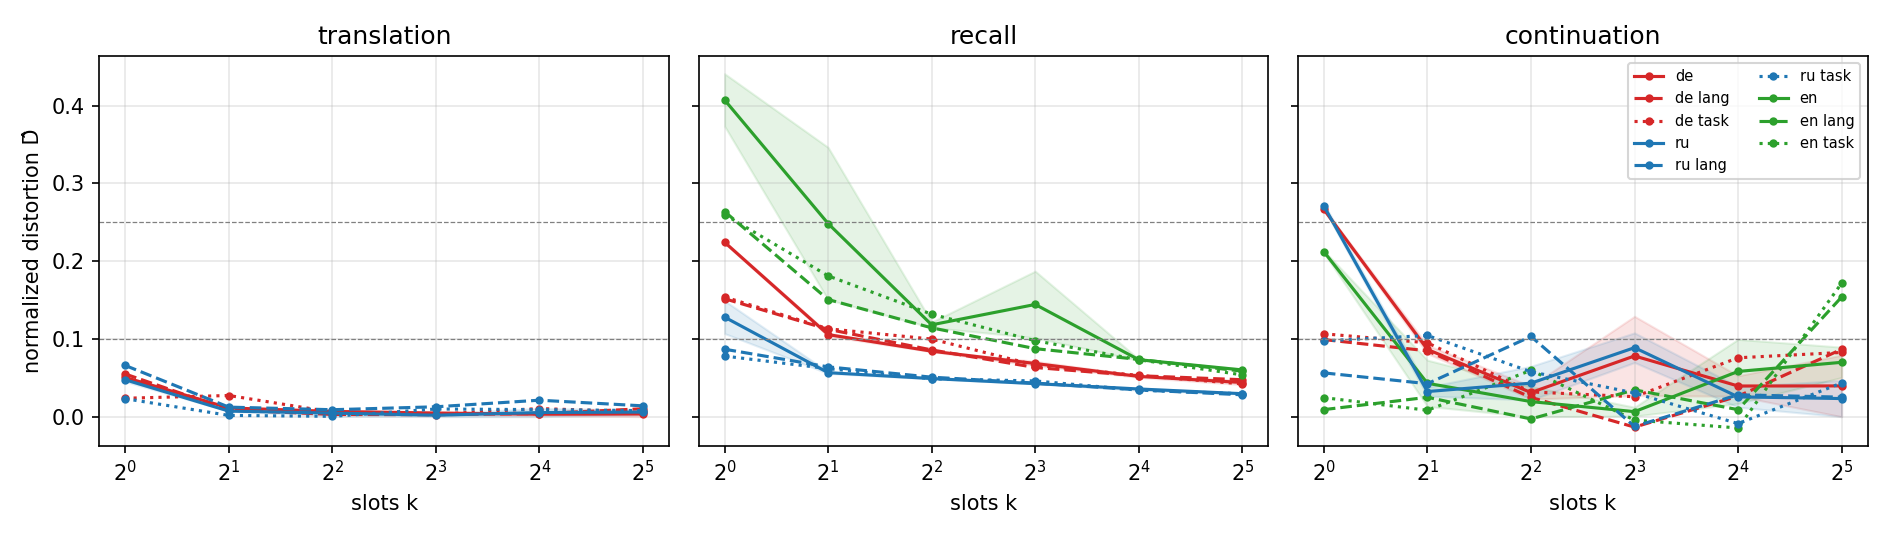
\includegraphics[width=\textwidth]{curves.png}
\caption{Normalised distortion against the number of slots, Design~A, seed means with the seed range shaded. Dashed lines mark the operating points; line style is the conditioning format. Continuation (right) is noise: its floor lies within 0.10--0.16 bits per token of the no-prefix loss.}
\label{fig:curves}
\end{figure}

Figure~\ref{fig:curves} shows $\Dh$ against $k$. Translation reaches $\Dh\le0.10$ with one slot in every language and conditioning and is flat from there. Recall keeps improving to $k=32$ on Russian and German with the budget binding: a 3000-step run on \cell{recall-ru} at $k=8$ moves $\Dh$ from 0.043 to 0.032 and is still falling. Continuation is excluded from every headline claim because its floor lies within 0.10--0.16 bits per token of the no-prefix loss, below the seed variation. Seed gaps are below 0.011 on translation, 0.042 on \cell{recall-ru} and \cell{recall-de}, and 0.20 on \cell{recall-en}. Table~\ref{tab:kstar} gives $k^\ast$.

\begin{table}[t]
\centering\small
\begin{tabular}{lccc}
\toprule
cell & $k^\ast(0.25)$ & $k^\ast(0.10)$ & $k^\ast(0.05)$, expl. \\
\midrule
translation-ru & 1 & 1 & 1 \\
translation-de & 1 & 1 & 2 \\
recall-ru & 1 & 2 & 4 \\
recall-de & 1 & 4 & 32 \\
recall-en & 2 & 16 & not reached \\
\bottomrule
\end{tabular}
\caption{Slot complexity: the smallest $k$ whose seed-mean $\Dh$ reaches the level.}
\label{tab:kstar}
\end{table}

Two observations make the slot count unusable as a description length. First, the natural-language prompt, scored as a context with no prefix, is far worse than one trained slot: on recall it leaves $\Dh$ at 0.91--0.96 where one slot leaves 0.13--0.41; on translation 0.12--0.20 against 0.05. One vector of 1,536 numbers carries more than an instruction, so a token is not a unit of information. Second, conditioning saves little on the slot axis: giving the language or the task changes $k^\ast(0.10)$ in none of the translation cells and in two recall cells (\cell{recall-ru} 2 to 1, \cell{recall-en} 16 to 8, for either conditioning). The savings $\Delta k_{\text{lang}}$ and $\Delta k_{\text{task}}$ average 1.8 slots each over the measurable cells, with 8 of those 9 slots from \cell{recall-en}. The slot axis cannot distinguish telling the model the language from telling it the task; the bit axis can.

\subsection{Description length in bits}\label{sec:bits}
\begin{figure}[t]
\centering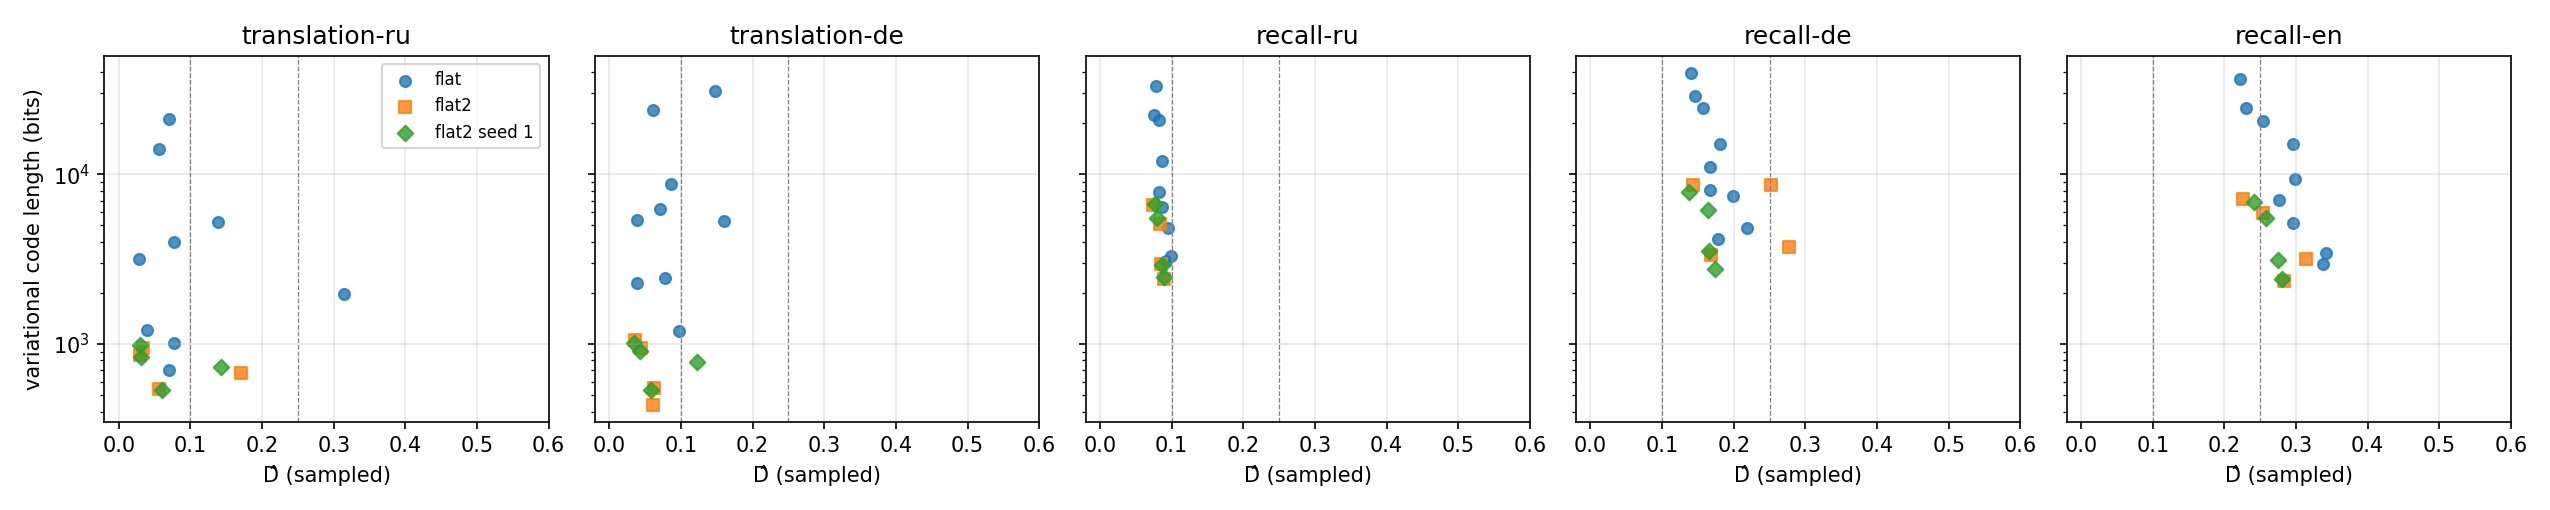
\includegraphics[width=\textwidth]{frontier.png}
\caption{Rate against distortion for every variational run, per cell. Circles: preregistered protocol; squares: corrected protocol. Distortion is scored on posterior samples.}
\label{fig:frontier}
\end{figure}

\begin{table}[t]
\centering\small
\setlength{\tabcolsep}{4pt}
\begin{tabular}{lrrrr}
\toprule
 & \multicolumn{2}{c}{corrected (flat2)} & best & prereg. \\
cell & $\Dh\le0.10$ & $\Dh\le0.25$ & $\Dh$ & $\Dh\le0.25$ \\
\midrule
translation-de & 436 & 436 & 0.036 & 1,194 \\
translation-ru & 542 & 542 & 0.030 & 699 \\
recall-ru & 2,419 & 2,419 & 0.075 & 3,101 \\
recall-de & --- & 3,343 & 0.143 & 4,168 \\
recall-en & --- & 7,155 & 0.226 & 24,686 \\
\bottomrule
\end{tabular}
\caption{Headline frontier: the smallest code length in bits among runs reaching each operating point, under the corrected protocol, with the best distortion any corrected run reaches and the preregistered protocol's value at 0.25.}
\label{tab:frontier}
\end{table}

Table~\ref{tab:frontier} is the headline. A translation program costs about 500 bits. A Russian recall program costs five times that; German and English recall do not reach 10\% excess loss within the budget and cost 3,300 and 7,200 bits at 25\%. Bootstrap intervals over test examples are narrow: the gain over the no-prefix model of the $\Dh\le0.10$ frontier runs, evaluated at the posterior mean (per-example bits are stored for the mean only), is $0.52\pm0.01$ bits per token on \cell{translation-ru}, $0.50\pm0.03$ on \cell{translation-de} and $5.69\pm0.07$ on \cell{recall-ru}.

The ordering across tasks within a language follows the learning gap $L_{\text{none}}-L_{\text{floor}}$ (recall 3.5--6.2 bits per token, translation 0.6--0.9), as hypothesised. The ordering across languages does not follow exposure: English recall is the dearest program, not the cheapest, in slots and in bits, and the result survives restricting the three recall test sets to the 4,212 items they share ($\Dh$ at $k=4$: ru 0.049, de 0.079, en 0.122). The English LoRA floor is also the worst of the three (2.58 bits per token against 1.10 for Russian), so what is dear in English is not the language but the facts mLAMA asks about in English.

\subsection{Neither nesting is cheaper, and sharing does not compress}\label{sec:hier}
\begin{figure}[t]
\centering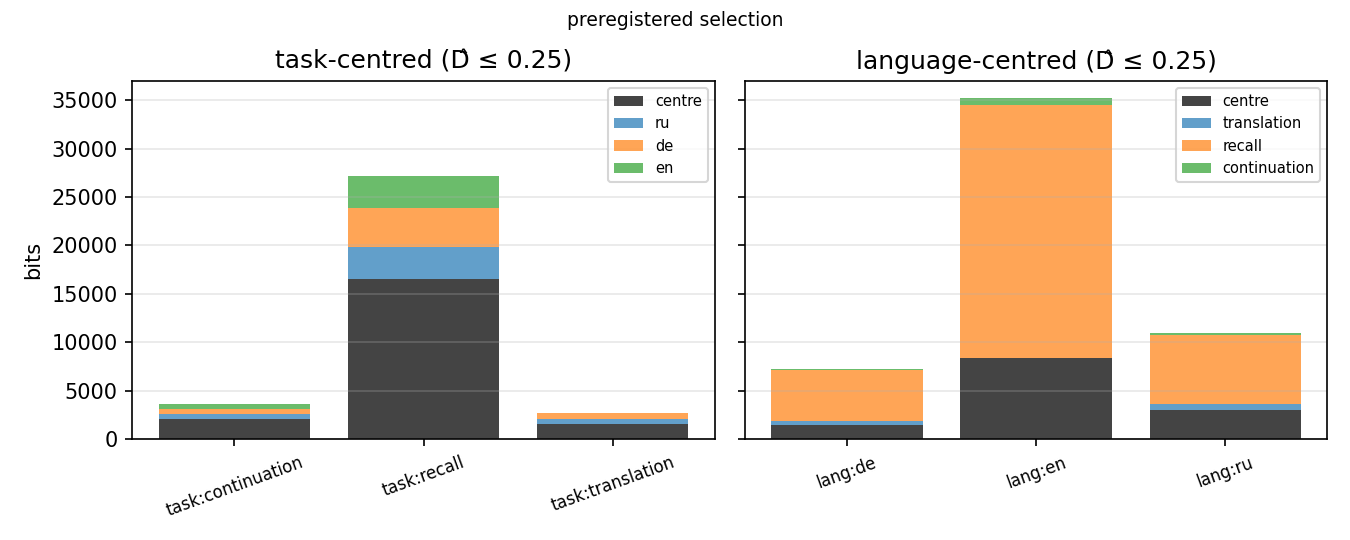
\includegraphics[width=0.85\textwidth]{hier_bars.png}
\caption{Code length at $\Dh\le0.25$ under the two nestings: the centre is paid once per group, each deviation once per member; the cheapest run whose members all reach the level.}
\label{fig:hier}
\end{figure}

\begin{table}[t]
\centering\small
\begin{tabular}{llr}
\toprule
code for all eight cells, $\Dh\le0.25$ & protocol & bits \\
\midrule
centre per task + language deviations & prereg.\ selection & 33,500 \\
eight independent programs & prereg. & 37,600 \\
centre per language + task deviations & prereg.\ selection & 53,500 \\
centre per task + language deviations & corrected & 26,700 \\
centre per language + task deviations & corrected & not reached (ru, de: 8,900) \\
eight independent programs & corrected & 17,600 \\
\bottomrule
\end{tabular}
\caption{Three codes for the same eight cells under both protocols. The corrected independent row uses flat2 on the five measurable cells and the preregistered runs on continuation; under the corrected protocol the language-centred hierarchy does not get \cell{recall-en} below 0.25 within the grid, so only its Russian and German groups are summed.}
\label{tab:codes}
\end{table}

Figure~\ref{fig:hier} and Table~\ref{tab:codes} compare the codes at $\Dh\le0.25$, the only level every cell reaches. Under the preregistered rule grouping by task costs 37\% less than grouping by language, and the task-centred code is 11\% cheaper than eight independent programs. Neither margin survives the corrected protocol, with both sides selected on the objective and scored on samples; both were selection artefacts of the kind described in Section~\ref{sec:opt}. Sharing does not compress: the task-centred hierarchy costs 26,700 bits against 17,600 for independent programs, a factor of 1.5. Table~\ref{tab:groups} gives the comparison per group: the task-centred hierarchy is at parity on translation and costs 1.9 times the independent programs on recall; the language-centred hierarchy is at parity on Russian and German and fails on English. At matched $(k,\beta)$ a hierarchy costs 0.94--1.5 times the sum of the flat2 runs with the same hyper-parameters, with worst-member distortion within 0.03 of the independent runs either way at six of the eight grid points and worse by 0.05--0.28 at the other two, so the shared centre buys nothing; the frontier comparison then adds the cost of one $\beta$ for every member. On recall the only task-centred run in which all three languages reach 0.25 is $(k,\beta)=(4,1)$, whose centre alone (14,600 bits) costs more than the three independent programs together, and the factor 1.93 decomposes as 1.12 (the matched excess at that point, 24,972 against 22,360) times 1.73 (one $\beta$ for all members, 22,360 against 12,917). Nor is either nesting cheaper than the other: at matched $(k,\beta)$ the language-centred code costs 0.88--1.24 times the task-centred one over all eight cells, at worse worst-member distortion in three of the four grid points and better in the fourth (Table~\ref{tab:nestings}). The 37\% gap of the preregistered runs came from language-centred recall deviations of 5,300--26,200 bits, which the corrected protocol brings down to 3,200--3,400 for Russian and German.

\begin{table}[t]
\centering\small
\begin{tabular}{lrrr}
\toprule
group, $\Dh\le0.25$ & hierarchy, corrected $(k,\beta)$ & independent, corrected & ratio \\
\midrule
translation (ru, de) & 1,029 (4, 3) & 978 & 1.05 \\
recall (ru, de, en) & 24,972 (4, 1) & 12,917 & 1.93 \\
continuation (ru, de, en; unmeasurable) & 667 (4, 3) & 3,724 (flat) & 0.18 \\
\midrule
Russian (translation, recall, continuation) & 4,353 (2, 3) & 4,204 & 1.04 \\
German (translation, recall, continuation) & 4,560 (2, 3) & 4,227 & 1.08 \\
English (recall, continuation) & not reached & 9,188 & -- \\
\bottomrule
\end{tabular}
\caption{Task-centred (top) and language-centred (bottom) hierarchies against independent programs per group under the corrected protocol; the independent continuation values are from the preregistered flat runs.}
\label{tab:groups}
\end{table}

\begin{table}[t]
\centering\small
\begin{tabular}{lrrr}
\toprule
$(k,\beta)$ & task-centred, bits (worst $\Dh$) & language-centred, bits (worst $\Dh$) & ratio \\
\midrule
(2, 1) & 24,591 (0.28) & 30,448 (0.59) & 1.24 \\
(2, 3) & 12,693 (0.56) & 11,182 (0.48) & 0.88 \\
(4, 1) & 28,659 (0.23) & 30,532 (0.28) & 1.07 \\
(4, 3) & 11,180 (0.28) & 13,396 (0.37) & 1.20 \\
\bottomrule
\end{tabular}
\caption{The two nestings at matched hyper-parameters under the corrected protocol: three centres plus eight deviations either way, summed over all eight cells, with the worst member distortion.}
\label{tab:nestings}
\end{table}

The per-member costs are symmetric under the corrected protocol. Given the translation centre (604 bits), a target language costs 225 (ru) or 200 (de) bits, 0.41--0.46 of a standalone program; given a language centre (830--900 bits), translation costs 201 (ru) or 257 (de). Given the recall centre (14,600 bits), a language costs 3,200--3,950 bits, 1.2--1.3 times a standalone Russian or German program; given a language centre, recall costs 3,200 (ru) or 3,400 (de), and for English no run reaches 0.25 (2,600 bits at 0.37, 6,500 at 0.28). Continuation given a language centre costs 60 bits. Under the preregistered rule the same quantities were 485 and 662 for a language given translation, 3,300--4,000 for a language given recall, and 440--630, 5,300--26,200 and 110--740 for translation, recall and continuation given a language; the asymmetry was in the optimiser. Recall is the program that cannot be shared with anything: it costs about 3,200 bits as a deviation from either kind of centre, and whichever group must carry it (the recall group, or the English group, whose recall deviation never reaches 0.25) is the expensive one. For translation alone the hierarchy is at best at parity: centre plus two deviations costs 1,029 bits at $\Dh\le0.10$ under the corrected protocol against 978 for two independent programs (2,733 against 1,893 under the preregistered rule); the centre costs more than either specialised program (604 against 542 and 436 bits) and each deviation less than half of one, so centre plus deviation cannot be cheaper. In bits, then, the task given the language costs 0.9--1.0 (ru, de) times the language given the task on recall and 0.9--1.3 on translation, where the preregistered rule had given 1.3--7.8 on recall; this agrees with the slot axis, where $\Delta k_{\text{lang}}=\Delta k_{\text{task}}$.

\subsection{Composition}\label{sec:compose}
\begin{figure}[t]
\centering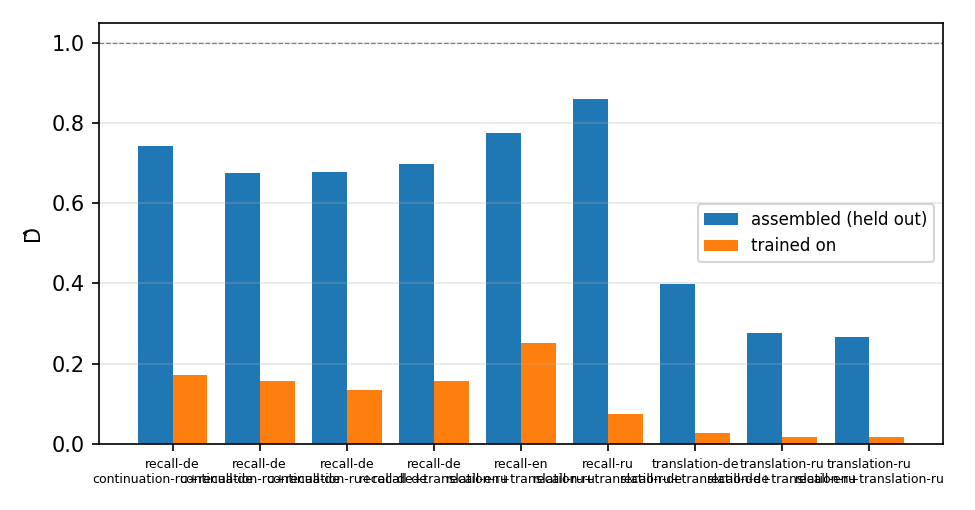
\includegraphics[width=0.8\textwidth]{compose.png}
\caption{Assembled (held-out) against trained-on $\Dh$ of tied task and language parts, per hold-out.}
\label{fig:compose}
\end{figure}
Six tied parts trained on every cell match Design~A at the same total slots on translation ($\Dh$ 0.017--0.027 against 0.005--0.007 at $2{+}2$) and cost about twice its distortion on recall (0.08--0.25 against 0.05--0.12). Assembled zero-shot for a held-out cell (Figure~\ref{fig:compose}), the parts close 60--73\% of the gap between no prefix and the floor on translation (three hold-outs over two cells, $\Dh$ 0.27--0.40) and 14--32\% on recall (six hold-outs over three cells, $\Dh$ 0.68--0.86). Task and language parts compose partially for translation and barely for recall.

\subsection{Distance between programs}\label{sec:distance}
\begin{figure}[t]
\centering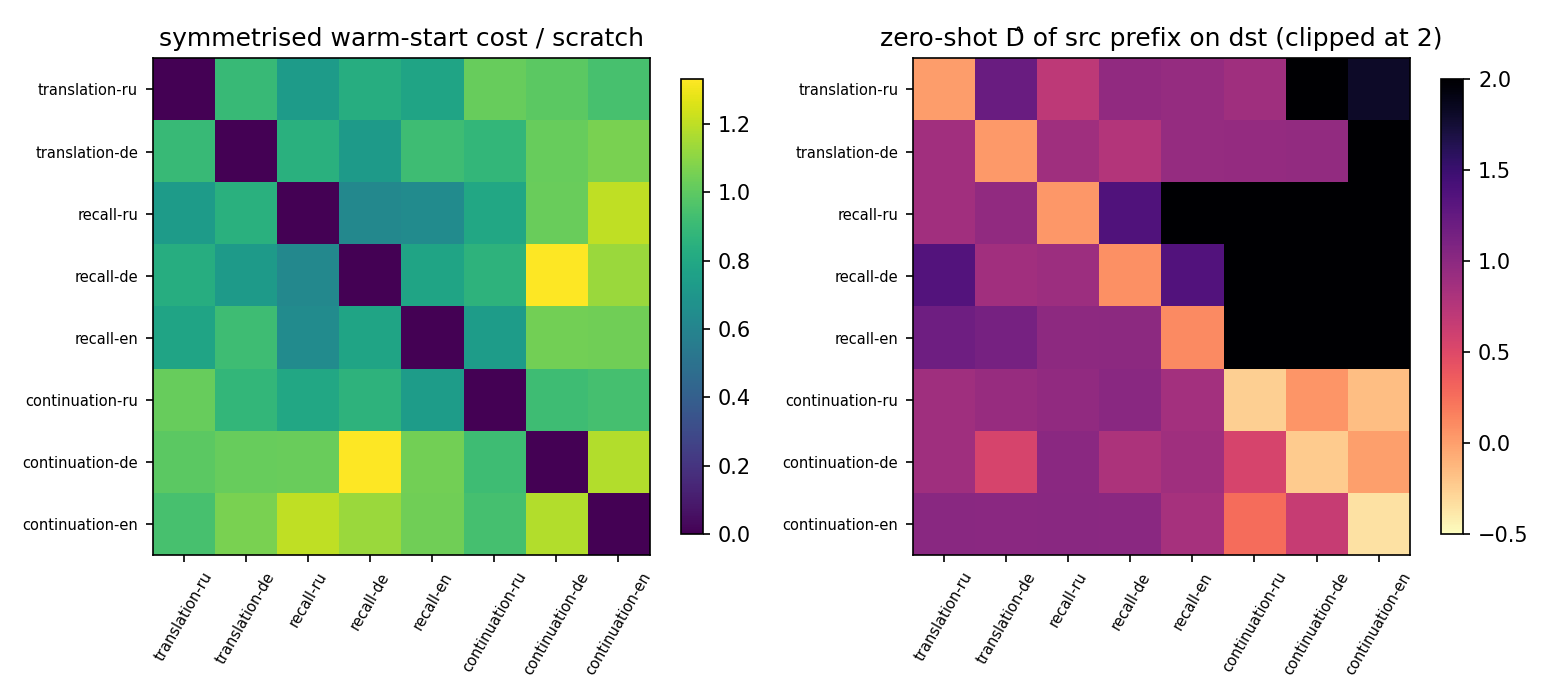
\includegraphics[width=0.95\textwidth]{distance.png}
\caption{Left: symmetrised warm-start learning cost divided by the from-scratch cost. Right: $\Dh$ of a trained prefix applied unchanged to another cell, clipped at 2.}
\label{fig:distance}
\end{figure}
Warm-starting from a prefix of the same task costs 0.85 of training from scratch; from the same language or an unrelated cell, 0.95 (Figure~\ref{fig:distance}, left). The silhouette of the task partition on the symmetrised distance is 0.004 and that of the language partition $-0.09$: the direction is the hypothesised one, the structure is absent, and with seven pairs per group at one seed the difference is not significant. The zero-shot block (right) is the strong signal: a prefix applied to any other cell is roughly as bad as, or worse than, no prefix ($\Dh$ 0.7--1.4, median 0.97, up to 2.5), and a recall prefix applied to continuation is catastrophic ($\Dh$ 5--25). The recall program overrides the model's default behaviour rather than adding to it.

\subsection{Where the program is read}\label{sec:mech}
\begin{figure}[t]
\centering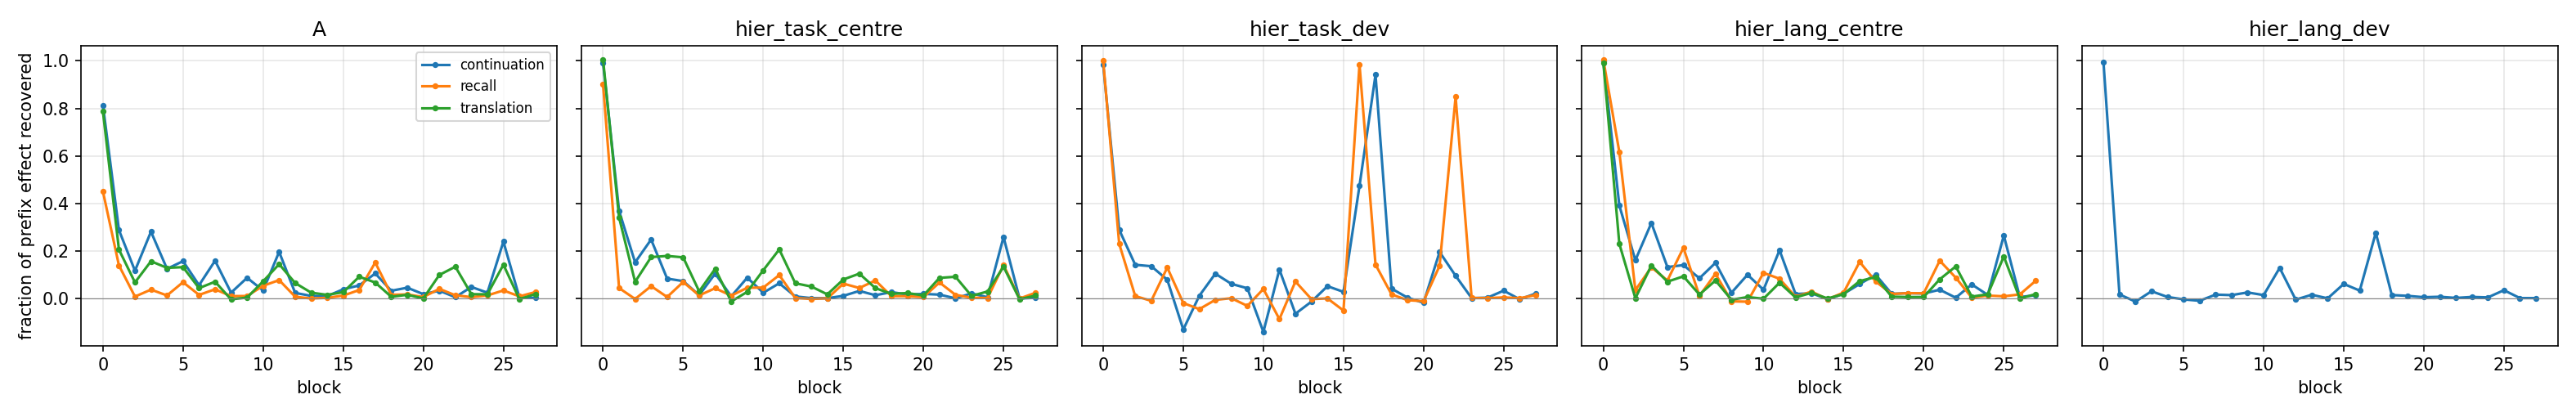
\includegraphics[width=\textwidth]{mechanism.png}
\caption{Fraction of a prefix's effect recovered by patching its positions into one block's attention input, mean over cells per task. Probes: \texttt{A} (Design~A, $k=4$); \texttt{hier\_task\_centre} and \texttt{hier\_task\_dev} (task centre; language deviation on top of it); \texttt{hier\_lang\_centre} and \texttt{hier\_lang\_dev} (language centre; task deviation on top of it). Fractions are undefined where the donor is not at least 0.1 bits per token better than the recipient.}
\label{fig:mech}
\end{figure}
Patching all blocks reproduces the donor exactly. Patching block~0 alone recovers 70--87\% of the effect for translation and 74--94\% for continuation, but only 36--58\% for recall, which has a secondary peak at block~17 and a smaller one at blocks 10--11 (Figure~\ref{fig:mech}, left). Single-block fractions summed over blocks come to 2.6 for translation and 3.0 for continuation, so their reading is redundant, but 1.3 for recall, which is close to additive. A translation program is copied into the token stream in the first block and not needed afterwards; a recall program is read in several places, deep in the network.

The block of maximal recovery is block~0 for every probe on every cell, so the peak does not separate the parts of a hierarchical prefix. The profiles do. The task centre is read early: on recall its mass over blocks 0--3 is 1.0 and over blocks 14--27 it is 0.5. The language deviation on top of it is read early and again deep: on recall 1.6 early and 1.9 late, with block~17 alone recovering 0.94 of the deviation's effect; on \cell{translation-de} 1.2 and 2.1, with blocks 16 and 22 recovering 0.99 and 0.85. The task deviation under a language centre behaves like the task centre (1.0 and 0.5). There is a depth split by prefix part, in the opposite direction to the language-early, task-middle expectation drawn from \citet{dumas2025separating}: the task part is read early, the language part early and late. One detail: the recall centre without its English deviation is worse than a random prefix on English, so the recall centre is a non-English program. Probing the corrected hierarchies ($k=4$, $\beta=1$) at their posterior means, which under that protocol are not the coded programs, leaves the hierarchical probes undefined on two to five of the eight cells; where they are defined the split replicates, with the task centre read early on recall (early 1.1, late 0.4) and the language deviation late (1.2, 1.9). A sampled version of the probe is implemented and not yet run.

\subsection{Input compressibility (exploratory)}
With the $k=4$ task prefix, one per-example vector replaces the input to within 10\% of the real-input loss on every cell but \cell{translation-ru}, which needs two; without the prefix, translation and continuation need two. There is no rate term on the vectors, so this is a slot count.

\section{The objective is right, the search is hard}\label{sec:opt}
\begin{figure}[t]
\centering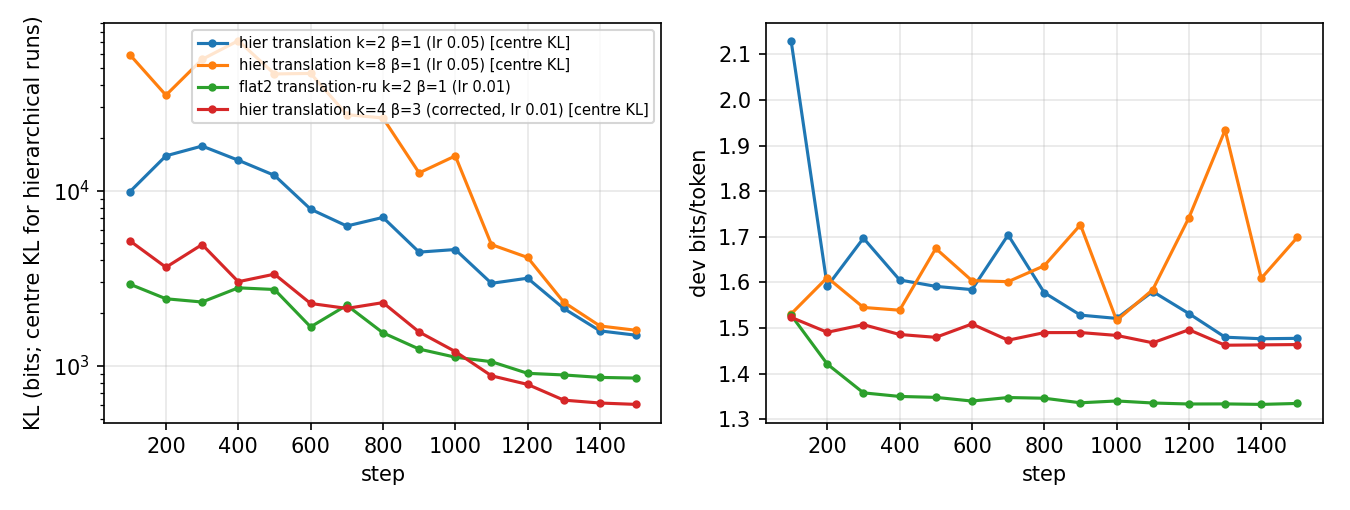
\includegraphics[width=0.85\textwidth]{trajectories.png}
\caption{Centre KL (hierarchical runs) or total KL (flat2) and development loss against step for two preregistered-protocol hierarchical runs and two corrected-protocol runs (flat2 and hierarchical).}
\label{fig:traj}
\end{figure}
The saved histories of the 27 task-grouped hierarchical runs show three things (Figure~\ref{fig:traj}). With learning rate 0.05, two prior standard deviations per Adam step, the centre KL overshoots early, peaking between steps 100 and 800 by an amount that grows with $k$: a median peak of 26,000 bits at $k=2$ (range 6,000--182,000) and 144,000 at $k=8$ (28,000--549,000), before the cosine schedule lets the KL term pull the means back. In the plotted translation runs the final centre rate is the same at $k=8$ as at $k=2$, but the posterior-mean distortion worsens late at $k=8$, so the distortion-only checkpoint rule selects a step where the rate is ten times the final one; across all runs the selected rate exceeds the final one by a median factor of 1.1--1.2 and up to 20. And the posterior mean is not the coded object: on translation at $\beta=3$ the mean scores $\Dh$ 0.35--0.56 in three of four runs while samples score 0.06--0.17.

The 12 task-grouped hierarchical runs under the corrected protocol show none of them: the centre KL peaks at step 150--200 at a median 3,600 ($k=2$) to 5,700 bits ($k=4$), 7--12 times lower, then falls monotonically, and the selected checkpoint is within 2\% of the final rate. The corrected protocol removes all three effects and lowers the measured frontier on every cell, by 22\% (\cell{translation-ru}, \cell{recall-ru}), 58--63\% (\cell{translation-de}), 20\% (\cell{recall-de}) and 71\% (\cell{recall-en}), with four runs per cell instead of nine, and the rates become monotone in $\beta$. \citet{shaw2026bridging} report that on a parity task the same objective reaches 870 bits from a hand-compiled initialisation but $2.8\times10^6$ bits from random initialisation, and leave the optimiser as the open problem. At this scale the gap closes mostly by selecting on the objective and stepping at the scale of the prior.

\section{Limitations}
Two seeds were preregistered; the second seed of the corrected variational protocol reproduces the frontier within 4\% on \cell{translation-ru}, \cell{recall-ru} and \cell{recall-en} and within 17--22\% on \cell{recall-de} and \cell{translation-de}, in opposite directions, with the same cell ordering (Table~\ref{tab:seeds}); the hierarchies and the distance matrix are one seed. The recall budget binds at 1500 steps, so recall rates are upper bounds. Continuation is unmeasurable because the frozen model already performs it. The variational protocol was corrected after the preregistered runs; both nestings were rerun under it on the flat2 grid ($k\in\{2,4\}$, $\beta\in\{1,3\}$, $\tau=1$), so the hierarchical comparisons are like for like but rest on four runs per group and one $\tau$. Under the corrected protocol every rate, flat or hierarchical, is still falling at the end of the 1500-step budget, so all are upper bounds; one run (English centre, $k=2$, $\beta=1$) selected a transient dip in the development loss at step 500. The mechanism probes patch attention inputs at the prefix positions; a residual-stream patch would answer a slightly different question. The exposure proxy for the language ordering was not available, so that comparison rests on orderings over three languages.

\section{Conclusion}
Counting tokens misreads a prompt's complexity; counting bits under a bits-back code does not, and at that currency a frozen 1.5B model needs about 500 bits to be told to translate and 2,400 or more to be told to recall facts. Those bits are not organised as a cheap modifier on a shared core in either direction: a language given a task costs what a task given a language costs, the two nestings cost the same, and a centre plus deviations costs no less than independent programs. The asymmetry is mechanistic: recall programs are language-specific, do not compose and are read deep, whereas translation programs are read in the first block. The measurement is only as good as the optimiser, and the largest single effect in this study is the one obtained by selecting checkpoints on the objective rather than on distortion. The research version runs the same code over the scale axis and twenty languages, charges $\log_2|k\text{-grid}|$ bits for the choice of $k$, adopts the per-column mixture prior of \citet{shaw2026bridging}, and gives each member of a hierarchy its own $\beta$, with three seeds.

\paragraph{Reproducibility}
Code, result tables, per-example bits, training histories and prefix checkpoints are in the repository (branch \texttt{prefixlab}); \texttt{notebooks/01\_figures.ipynb} regenerates every figure and table from the tables and \texttt{prereg.json}.

\bibliographystyle{plainnat}
\bibliography{refs}

\appendix
\section{Preregistered comparisons}
\begin{table}[h]
\centering\small
\begin{tabular}{p{0.06\textwidth}p{0.86\textwidth}}
\toprule
H1 & task ordering supported (recall far above translation); language ordering reversed on recall (English dearest), robust to common items; exposure proxy unavailable \\
H2 & equal on the slot axis (1.8 slots each, 8 of 9 from one cell); in bits, equal under the corrected protocol (task given language 0.9--1.0$\times$ language given task on recall, 0.9--1.3$\times$ on translation); the preregistered 1.3--7.8$\times$ asymmetry on recall does not replicate \\
H3 & translation composes partially (60--73\% of the gap zero-shot), recall barely (14--32\%); a shared centre saves no bits: under a common protocol the task-centred hierarchy costs 1.5$\times$ eight independent programs (parity on translation, 1.9$\times$ on recall) and the two nestings cost the same within 25\%; Chinese not run \\
H4 & silhouette 0.004 vs $-0.09$: task direction, no structure, not significant \\
H5 & block 0 for both; the language deviation is read again at blocks 16--17 and the task centre is not: a split by part, opposite in direction to the hypothesis \\
H6 & one vector suffices with the task prefix; per-token variant not computed; no rate term \\
\bottomrule
\end{tabular}
\caption{Outcome of each preregistered comparison.}
\end{table}

\section{Run inventory}
273 Design~A, baseline and floor rows (6 values of $k$, 2 seeds, 3 conditionings, 8 cells); 72 flat and 40 flat2 rows (two seeds); 144 hierarchical rows from 54 joint runs under the preregistered rule and 64 from 24 under the corrected protocol; 72 composition rows from 10 joint runs; 72 distance rows; 32 regime~2 rows; 1,120 mechanism rows; one 3000-step recall run. Training: 1500 steps, batch 16, AdamW, learning rate 0.05 (0.01 for flat2), 50 warm-up steps, cosine decay, gradient clip 1.0, development evaluation every 100 steps. LoRA floors: rank 16 on the attention projections, learning rate $2\times10^{-4}$, 1500 steps.
\begin{table}[h]
\centering\small
\begin{tabular}{lrrr}
\toprule
cell & seed 0, bits at 0.25 $(k,\beta)$ & seed 1, bits at 0.25 $(k,\beta)$ & ratio \\
\midrule
\cell{translation-ru} & 542 (4, 3) & 534 (4, 3) & 0.99 \\
\cell{translation-de} & 436 (2, 3) & 533 (4, 3) & 1.22 \\
\cell{recall-ru} & 2,419 (2, 3) & 2,486 (2, 3) & 1.03 \\
\cell{recall-de} & 3,343 (4, 3) & 2,783 (2, 3) & 0.83 \\
\cell{recall-en} & 7,155 (4, 1) & 6,850 (4, 1) & 0.96 \\
\bottomrule
\end{tabular}
\caption{Replication of the corrected-protocol frontier with a second seed; each seed's frontier is an independent replicate of the whole run grid. The binding level is 0.25 for \cell{recall-de} and \cell{recall-en} and 0.10 for the other cells, where the two levels coincide.}
\label{tab:seeds}
\end{table}

\end{document}
